% Created 2019-09-20 Пт 15:13
% Intended LaTeX compiler: pdflatex
\documentclass[11pt]{article}
\newcommand{\innp}[1]{\langle #1\rangle}
\usepackage{multirow}
\usepackage[utf8]{inputenc}
\usepackage[T1]{fontenc}
\usepackage{graphicx}
\usepackage{grffile}
\usepackage{longtable}
\usepackage{caption}
\usepackage{wrapfig}
\usepackage{rotating}
\usepackage[normalem]{ulem}
\usepackage{hyperref}
\usepackage{amsmath}
\usepackage{textcomp}
\usepackage{amssymb}
\usepackage{capt-of}
\usepackage{float}
\usepackage{graphicx}
\usepackage{hyperref}
\usepackage[T2A]{fontenc}
\usepackage[a4paper,left=3cm,top=2cm,right=1.5cm,bottom=2cm,marginparsep=7pt,marginparwidth=.6in]{geometry}
\usepackage{cmap}
\usepackage[russian]{babel}
\usepackage{xcolor}
\usepackage{listings}
\usepackage{makecell}
\author{АВТОР}
\date{\today}
\title{}
\hypersetup{
 pdfauthor={АВТОР},
 pdftitle={},
 pdfkeywords={},
 pdfsubject={},
 pdfcreator={Emacs 26.1 (Org mode 9.1.9)}, 
 pdflang={Russian}}
\setcounter{page}{2}
{\renewcommand{\arraystretch}{1.5}
\begin{document}
\tableofcontents
\pagebreak
\large
\section{Цель работы}
\begin{enumerate}
	\item Проверка основного закона динамики вращения.
	\item Проверка зависимости момента инерции от положения масс относительно
	оси вращения.
\end{enumerate}
\section{Требуемое оборудование}
\begin{enumerate}
	\item Лабораторный стенд для исследования вращательного движения.
	\item Цифровой секундомер.
\end{enumerate}
\section{Краткое теоретическое введение}
Груз m (см. рис. 1.) подвешен на нити, которая перекинута через
неподвижный блок Бл и намотана на ступицу Ст крестовины Кр. В ступице
закреплены четыре спицы Сп, на каждой из которых размещен груз–
утяжелитель m ут . Расстояние R утяжелителей от оси вращения крестовины
одинаково для всех утяжелителей. Это расстояние, можно изменять, изменяя
тем самым момент инерции крестовины с утяжелителями.
\begin{figure}[H]
	\centering
	\captionsetup{justification=centering}
	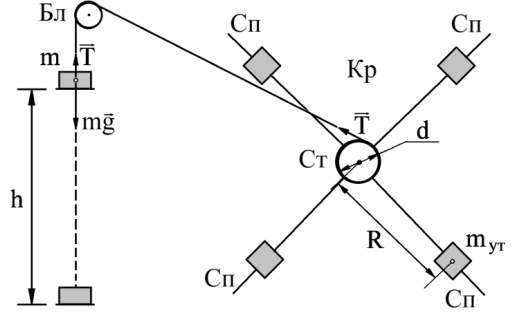
\includegraphics[width=300px]{../im1.png}
	\caption{Схема измерительного
стенда}
\end{figure}
~\\
Груз m, опускаясь, раскручивает крестовину. Если пренебречь силой
сопротивления воздуха, то груз движется равноускорено под действием
векторной суммы силы тяжести mg и силы T натяжения нити. Его ускорение a
определяется вторым законом Ньютона:
$$ma = mg - T \eqno(1)$$
Это ускорение можно вычислить по формуле
$$a = \frac{2h}{t^2} \eqno(2)$$
где h расстояние, пройденное грузом за время t от начала движения.\\
Нить не проскальзывает по ступице, поэтому угловое ускорение $\varepsilon$
крестовины согласовано с линейным ускорением груза. Это угловое ускорение
вычисляется по формуле
$$\varepsilon = \frac{2a}{d}\eqno(3)$$
где d диаметр ступицы.
Используя уравнение (1) выразим силу натяжения нити:
$$T = m(g-a) \eqno(4)$$
и найдем момент этой силы:
$$M = \frac{md}{2}(g-a) \eqno(5)$$
Предполагая, что кроме момента силы натяжения на раскручивание
крестовины влияет тормозящий момент силы трения, запишем основной закон
динамики вращения для крестовины в виде
$$I_{\varepsilon} = M - M_{\text{тр}} \eqno(6)$$
Здесь I момент инерции крестовины с утяжелителями.\\
В соответствии с теоремой Штейнера момент инерции крестовины зависит
от расстояния между центрами грузов и осью вращения по формуле
$$I = I_0 + 4m_{\text{уг}}R^2 \eqno(7)$$
где $I_0$ сумма моментов инерции стержней крестовины, момента инерции
ступицы и собственных центральных моментов утяжелителей.
\section{Данные об установке}
\begin{table}[H]
	\centering
	\large
	\caption{Данные об установке}
	\begin{tabular}{|c|c|}
		\hline
		Масса каретки & $(47,0 \pm 0,5) $ г\\
		\hline
		Масса шайбы & $(220,0 \pm 0,5) $ г\\
		\hline
		Масса грузов на крестовине & $(408,0 \pm 0,5) $ г\\
		\hline
		Расстояние первой риски от оси & $(57,0 \pm 0,5) $ мм\\
		\hline
		Расстояние между рисками & $(25,0 \pm 0,2) $ мм\\
		\hline
		Диаметр ступицы & $(46,0 \pm 0,5) $ мм\\
		\hline
		Диаметр груза на крестовине & $(40,0 \pm 0,5) $ мм\\
		\hline
		Высота груза & $(40,0 \pm 0,5) $ мм\\
		\hline
	\end{tabular}
\end{table}
\pagebreak
\section{Прямые измерения}
\begin{table}[htb]
	\centering
	\large
	\caption{Протокол измерений времени падения груза при разной массе груза и разном
		положении утяжелителей на крестовине}
	\begin{tabular}{|c|c|c|c|c|c|c|}
		\hline
		\multirow{2}{*}{\makecell{Масса\\груза,г}}& \multicolumn{6}{c|}{Положение утяжелителей}\\
		\cline{2-7}
		&1.риска&2.риска&3.риска&4.риска&5.риска&6.риска\\
		\hline
		\multirow{4}{*}{$m_1$} & $t_1 = 4,56$ & 4,99 & 6,08 & 7,18 & 7,75 & 8,60\\
		\cline{2-7}
		& $t_2 = 4,65$ & 5,08 & 5,92 & 7,05 & 7,94 & 8,70\\
		\cline{2-7}
		& $t_3 = 4,54$ & 5,16 & 5,90 & 7,22 & 7,78 & 8,72\\
		\cline{2-7}
		& $t_{\text{ср}} = 4,58;  \Delta t = 0,15$ & 5,08 & 5,97 & 7,15 & 7,82 & 8,67\\
		\hline
		\multirow{4}{*}{$m_2$} & $t_1 = 3,34$ & 3,93 & 4,55 & 5,30 & 5,98 & 6,48\\
		\cline{2-7}
		& $t_2 = 3,42$ & 3,86 & 4,42 & 5,29 & 5,98 & 6,58\\
		\cline{2-7}
		& $t_3 = 3,37$ & 3,83 & 4,38 & 5,28 & 5,96 & 6,31\\
		\cline{2-7}
		& $t_{\text{ср}} = 3,37$ & 3,87 & 4,55 & 5,29 & 5,97 & 6,46\\
		\hline
		\multirow{4}{*}{$m_3$} & $t_1 = 2,76$ & 3,27 & 3,62 & 4,21 & 4,90 & 5,53\\
		\cline{2-7}
		& $t_2 = 2,68$ & 3,17 & 3,64 & 4,36 & 4,94 & 5,47\\
		\cline{2-7}
		& $t_3 = 2,73$ & 3,32 & 3,69 & 4,34 & 4,97 & 5,30\\
		\cline{2-7}
		& $t_{\text{ср}}  = 2,73$ & 3,25 & 3,65 & 4,30 & 4,94 & 5,43\\
		\hline
		\multirow{4}{*}{$m_2$} & $t_1 = 2,49$ & 2,83 & 3,19 & 3,85 & 4,28 & 4,85\\
		\cline{2-7}
		& $t_2 = 2,35$ & 2,82 & 3,23 & 3,89 & 4,32 & 4,87\\
		\cline{2-7}
		& $t_3 = 2,49$ & 2,88 & 3,21 & 3,80 & 4,29 & 4,61\\
		\cline{2-7}
		& $t_{\text{ср}} = 2,44$ & 2,84 & 3,21 & 3,85 & 4,30 & 4,78\\
		\hline
	\end{tabular}
\end{table}
~\\
Настоящий протокол приведен в Приложении 3.\\\\
Посчитана абсолютная погрешность первого $t_{\text{ср}}$ по формуле:
$$\Delta t = \sqrt{{\Delta_{\overline{x}}^2} + {\left(\frac{2}{3} \Delta_{\text{иt}}\right)}^2} \eqno(8)$$
где $\Delta_{\overline{x}^2}$ - случайная погрешность, а $\Delta_{\text{иt}}$ - инструментальная (принята за 0,005, т.к. измерения проводились с цифрового секундомера с ценой деления 0,01 c)
\section{Задание 1}
Используя найденные значения $t_{\text{ср}}$ рассчитать ускорение $a$ груза, угловое
ускорение$\varepsilon$ крестовины и момент $M$ силы натяжения нити. Результаты
оформить в виде таблицы. Для первых значений $a$, $\varepsilon$ и $M$ вычислить их
погрешности и записать соответствующие доверительные интервалы.
\pagebreak
\begin{table}[H]
	\centering
	\small
	\caption{Рассчитанные значения ускорения груза, углового ускорения крестовины и момента силы натяжения нити}
	\begin{tabular}{|c|c|c|c|c|c|c|}
		\hline
		\multirow{2}{*}{\makecell{Масса\\груза,г}}& \multicolumn{6}{c|}{Положение утяжелителей}\\
		\cline{2-7}
		&1.риска&2.риска&3.риска&4.риска&5.риска&6.риска\\
		\hline
		\multirow{3}{*}{$m_1$} & $a = (0,067 \pm 4 \cdot 10^{-3})$ & $0,054$ & $0,039$ & $0,027$ & $0,023 $ & $ 0,019$\\
		\cline{2-7}
		& $\varepsilon = (2,91 \pm 1,8 \cdot 10^{-1})$ & $ 2,35$ & $1,70$ & $ 1,18$ & $1,00$ & $0,83$\\
		\cline{2-7}
		& $M = (0,0493 \pm 5 \cdot 10^{-4})$ & $0,0494$ & $0,0494$ & $0,0405$ & $0,0495$ & $0,0495$\\
		\hline
		\multirow{3}{*}{$m_2$} & $a = 0,123$ & $0,093$ & $0,068$ & $0,050$ & $0,039$ & $0,034 $\\
		\cline{2-7}
		& $\varepsilon = 5,35$ & $4,04$ & $2,96$ & $2,17$ & $1,70$ & $1,48$\\
		\cline{2-7}
		& $M = 0,0980$ & $0,0983$ & $0,0986$ & $0,0987$ & $0,0989$ & $0,0989$\\
		\hline
		\multirow{3}{*}{$m_3$} & $a = 0,188$ & $0,133$ & $0,105$ & $0,076$ & $0,057$ & $0,047$\\
		\cline{2-7}
		& $\varepsilon = 8,17$ & $5,78$ & $4,57$ & $3,30$ & $2,48$ & $2,04$\\
		\cline{2-7}
		& $M = 0,1460$ & $0,1469$ & $0,1473$ & $0,1477$ & $0,1480$ & $0,1482$\\
		\hline
		\multirow{3}{*}{$m_4$} & $a = 0,235$ & $0,174$ & $0,136$ & $0,094$ & $0,076$ & $0,061$\\
		\cline{2-7}
		& $\varepsilon = 10,22$ & $7,57$ & $5,91$ & $4,09$ & $3,30$ & $2,65$\\
		\cline{2-7}
		& $M = 0,1937$ & $0,1950$ & $0,1957$ & $0,1966$ & $0,1970$ & $0,1973$\\
		\hline
	\end{tabular}
\end{table}
~\\
Считаем абсолютную погрешность ускорения груза по формуле:
$$\Delta a = a \cdot \sqrt{\left(1 \cdot\frac{\Delta h}{h}\right)^2 + {\left(-2\cdot\frac{\Delta t}{t}\right)}^2} \eqno(9)$$
Углового ускорения ступицы:
$$\Delta \varepsilon =  \varepsilon \cdot \sqrt{\left(1 \cdot\frac{\Delta a}{a}\right)^2 + {\left(-1\cdot\frac{\Delta d}{d}\right)}^2} \eqno(10)$$
Момента силы натяжения нити:
$$\Delta M = M \cdot \sqrt{\left(1 \cdot\frac{\Delta m}{m}\right)^2 + {\left(1\cdot\frac{\Delta d}{d}\right)}^2 + {\left(1\cdot\frac{\Delta (g-a)}{(g-a)}\right)}^2} \eqno(11)$$
Абсолютные погрешности считаются как погрешности косвенных измерений Способом 2 из учебно-методического пособия "Физика Обработка эксперементальных данных".
Для нахождения $\Delta M $ $\Delta (g-a)$ принято за $\Delta a$, т.к. погрешность табличной константы $g$ не учитывается. $g$  взята точностью $a$.
\pagebreak
\section{Задание 2}
Для каждого положения утяжелителей на основе Таблицы 3 отметить точки на графиках и построить теоритические зависимости $M(\varepsilon)$ методом наименьших квадратов (МНК). Для первого графика отметить погрешности.\\\\
Теоритическая зависимость описывается уравнением:
$$M = M_{\text{тр}} + I\varepsilon \eqno(12)$$
Формулы расчёта коэффициентов по МНК:
$$I = \frac{\sum(\varepsilon_i-\overline{\varepsilon})(M_i-\overline{M})}{\sum{(\varepsilon_i-\overline{\varepsilon})}^2} \eqno(13)$$
$$M_{\text{тр}} = \overline{M} - I\overline{\varepsilon} \eqno(14)$$
где $\overline{\varepsilon}$ и $\overline{M}$ соотвественно средние $\varepsilon$ и $M$.
\begin{table}[H]
	\centering
	\large
	\caption{Коэффициенты для Графиков 1-6}
	\begin{tabular}{|c|c|c|}
		\hline
		& $I$, кг $\cdot$ м$^2$&$M_{\text{тр}}$, Н $\cdot$ м\\
		\hline
		График 1 & $0,019$&$-4,74 \cdot 10^{-3}$\\
		\hline
		График 2 & $0,028$&$-1,50 \cdot 10^{-2}$\\
		\hline
		График 3 & $0,034$&$-7,0 \cdot 10^{-2}$\\
		\hline
		График 4 & $0,052$&$-2,0 \cdot 10^{-2}$\\
		\hline
		График 5 & $0,065$&$-1,7 \cdot 10^{-2}$\\
		\hline
		График 6 & $0,082$&$-2,0 \cdot 10^{-2}$\\
		\hline
	\end{tabular}
\end{table}
~\\
График 1 соотвествует положению утяжелителей на 1 риске, График 6 - на 6 риске.
Графики представлены в Приложении 1.
\section{Задание 3}
Для каждого положения утяжелителей найти расстояние $R$ (см Рис.1) между осью $O$ и центром вращения $C$ по формуле (15). Вычислить $R^2$.\\
Объединить значения $R$, $R^2$, $I$ в таблицу и на основе этой таблицы построить график $I(R^2)$.\\
На основе экспериментальных значений $I$ и $R^2$ с помощью МНК
определить значения $I_0$ и $m_{\text{ут}}$ из теоретической зависимости (формула (7)), а так же их погрешности $\Delta I_0$ и $\Delta m_{\text{ут}}$.\\
Построить график теоретической зависимости.
$$R = l_1 + (n-1)l_0 + \frac{1}{2}b \eqno(15)$$
\pagebreak
~\\
В формуле (15) $l_1$  - расстояние от оси вращения до первой риски; $n$ - номер риски,
на которой установлены утяжелители; $l_0$ - расстояние между соседним
рисками; $b$ - размер утяжелителя вдоль спицы.
\begin{table}[H]
	\centering
	\large
	\caption{Рассчитанные значения $R$, $R^2$ и $I$}
	\begin{tabular}{|c|c|c|c|}
		\hline
		Положение утяжелителя& $R$, м & $R^2$, м$^2$ & $I$, кг $\cdot$ м$^2$\\
		\hline
		1.риска & $0,077$& $0,006$& $0,019$\\
		\hline
		2.риска & $0,102$ & $0,010$& $0,028$\\
		\hline
		3.риска & $0,127$& $0,016$& $0,034$\\
		\hline
		4.риска & $0,152$& $0,023$& $0,052$\\
		\hline
		5.риска & $0,177$& $0,031$& $0,065$\\
		\hline
		6.риска & $0,202$& $0,041$& $0,082$\\
		\hline
	\end{tabular}
\end{table}
Для расчета коэффициентов теоретической зависимости $I(R^2)$ использовались формулы, аналогичные формулам (12) и (13).\\\\
$I_0 = 0,008$ кг $\cdot$ м$^2$\\\\
$4m_{\text{ут}} = 1,811$ кг $=> m_{\text{ут}} = 0,453$ кг\\\\
Расчитаем среднеквадратичное отклонение (СКО) для найденных значений:
$$d_i = {I}_i - (I_0 + 4m_{\text{ут}}{R^2}_i); \qquad D = \sum({R^2}_i - \overline{R^2}) \eqno(16)$$ 
$$S_{m_{\text{ут}}} = \sqrt{\frac{\sum d_i^2}{D \cdot 4}}; \qquad S_{I_0} = \sqrt{\left(\frac{1}{6}+\frac{{\overline{R^2}}^2}{D}\right)\frac{\sum d_i^2}{4}} \eqno(17)$$\\\\
$S_{m_{\text{ут}}} = 7 \cdot 10^{-2}; \qquad S_{I_0} = 1,7 \cdot 10^{-3}$\\\\
Рассчитаем случайную погрешность для доверительной вероятности 0,95:\\\\
$\Delta{m_{\text{ут}}} = 1,8 \cdot 10^{-1}; \qquad \Delta{I_0} = 4,4 \cdot 10^{-3}$\\\\
График 7 зависимости $I(R^2)$ представлен в Приложении 2.
\section{Вывод}
По результатам измерений построены графики зависимости момента силы от углового ускорения, по которому найден момент инерции крестовины. Построен график зависимости момента инерции крестовины от квадрата расстояний грузов от центра крестовины. Найдена масса грузов на крестовине $(0,453 \pm 1,8 \cdot 10^{-1})$, которая совпадает с данной в Таблице 1 с учетом погрешности.
\end{document}